\chapter{Mutual Information}
\label{chapter:intro}
相互資訊(Mutual Information,MI),是衡量兩個隨機變量之間關係性存在和強度的指標。它通過查看另一個隨機變量來量化關於一個隨機變量中預期的“信息量”。也可以說假設有A和B兩事件,在B已發生的情況下,而A會發生所能提供的資訊。相互資訊不限於實值隨機變量和線性相關,並確定兩個變量之間的聯合分佈和邊際分佈的乘積的相似程度。

%%\begin{equation}
%%%\label{eqn:MI}
%%    \textbf{i}(x,y)=\sum_{y\in Y}^{}\sum_{x\in X}^{}p(x,y)log(\frac{p(x,y)}{p(x),p(y)})
%%\end{equation}


$$\textbf{i}(x,y)=\sum_{y\in Y}^{}\sum_{x\in X}^{}p(x,y)log(\frac{p(x,y)}{p(x),p(y)})$$

        兩個屬性 X 和 Y 之間的相互信息,表示為 I(X, Y),它可以衡量對一個 屬性值的了解,能減少有關另一個屬性值的不確定性。如果 I(X, Y)很大,則可能存在一些相關性很強的連接在X和Y之間。

        \begin{figure}[h]
            \centering
            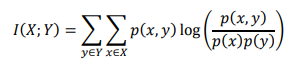
\includegraphics[width=10cm]{./pic/MI.PNG}
            \caption{MI示意圖}
            \label{fig:MI}
        \end{figure}

